% !TEX encoding = UTF-8
% !TEX TS-program = pdflatex
% !TEX root = ../tesi.tex

%**************************************************************
\chapter{Le 6 W}
\label{cap:le 6 w}
Nelle sezioni seguenti vengono analizzate le cosiddette 6 W, partendo dalla Homepage e poi analizzando le altre pagine del sito. Due di esse ("Mercatino" e "I Nostri Atleti") sono ancora in costruzione al momento in cui ho fatto l'analisi del sito e pertanto non verranno prese in considerazione.

%**************************************************************
\section{Homepage}
\begin{figure}[ht]
    \centering
    \includegraphics[scale=0.2]{./immagini/homepage}
    \caption [Homepage del sito]{Homepage del sito \siteName}
\end{figure}
La prima pagina che si vede quando si visita il sito è la Homepage (ovviamente). Tuttavia questa pagina è tutto tranne che una homepage: dovrebbe essere il cuore del sito e deve essere gestita come un testo giornalistico, quindi deve rispettare le 6W. Ciò che vede l'utente quando entra sono due grandi banner pubblicitari: il "vero" sito inizia dopo uno scroll di una pagina. Per poter rispondere (in parte) alle 6 W è necessario quindi scrollare di una pagina.

\begin{figure}[ht] 
    \centering
    \includegraphics[width=.49\textwidth]{./immagini/homepage2}\hfil
    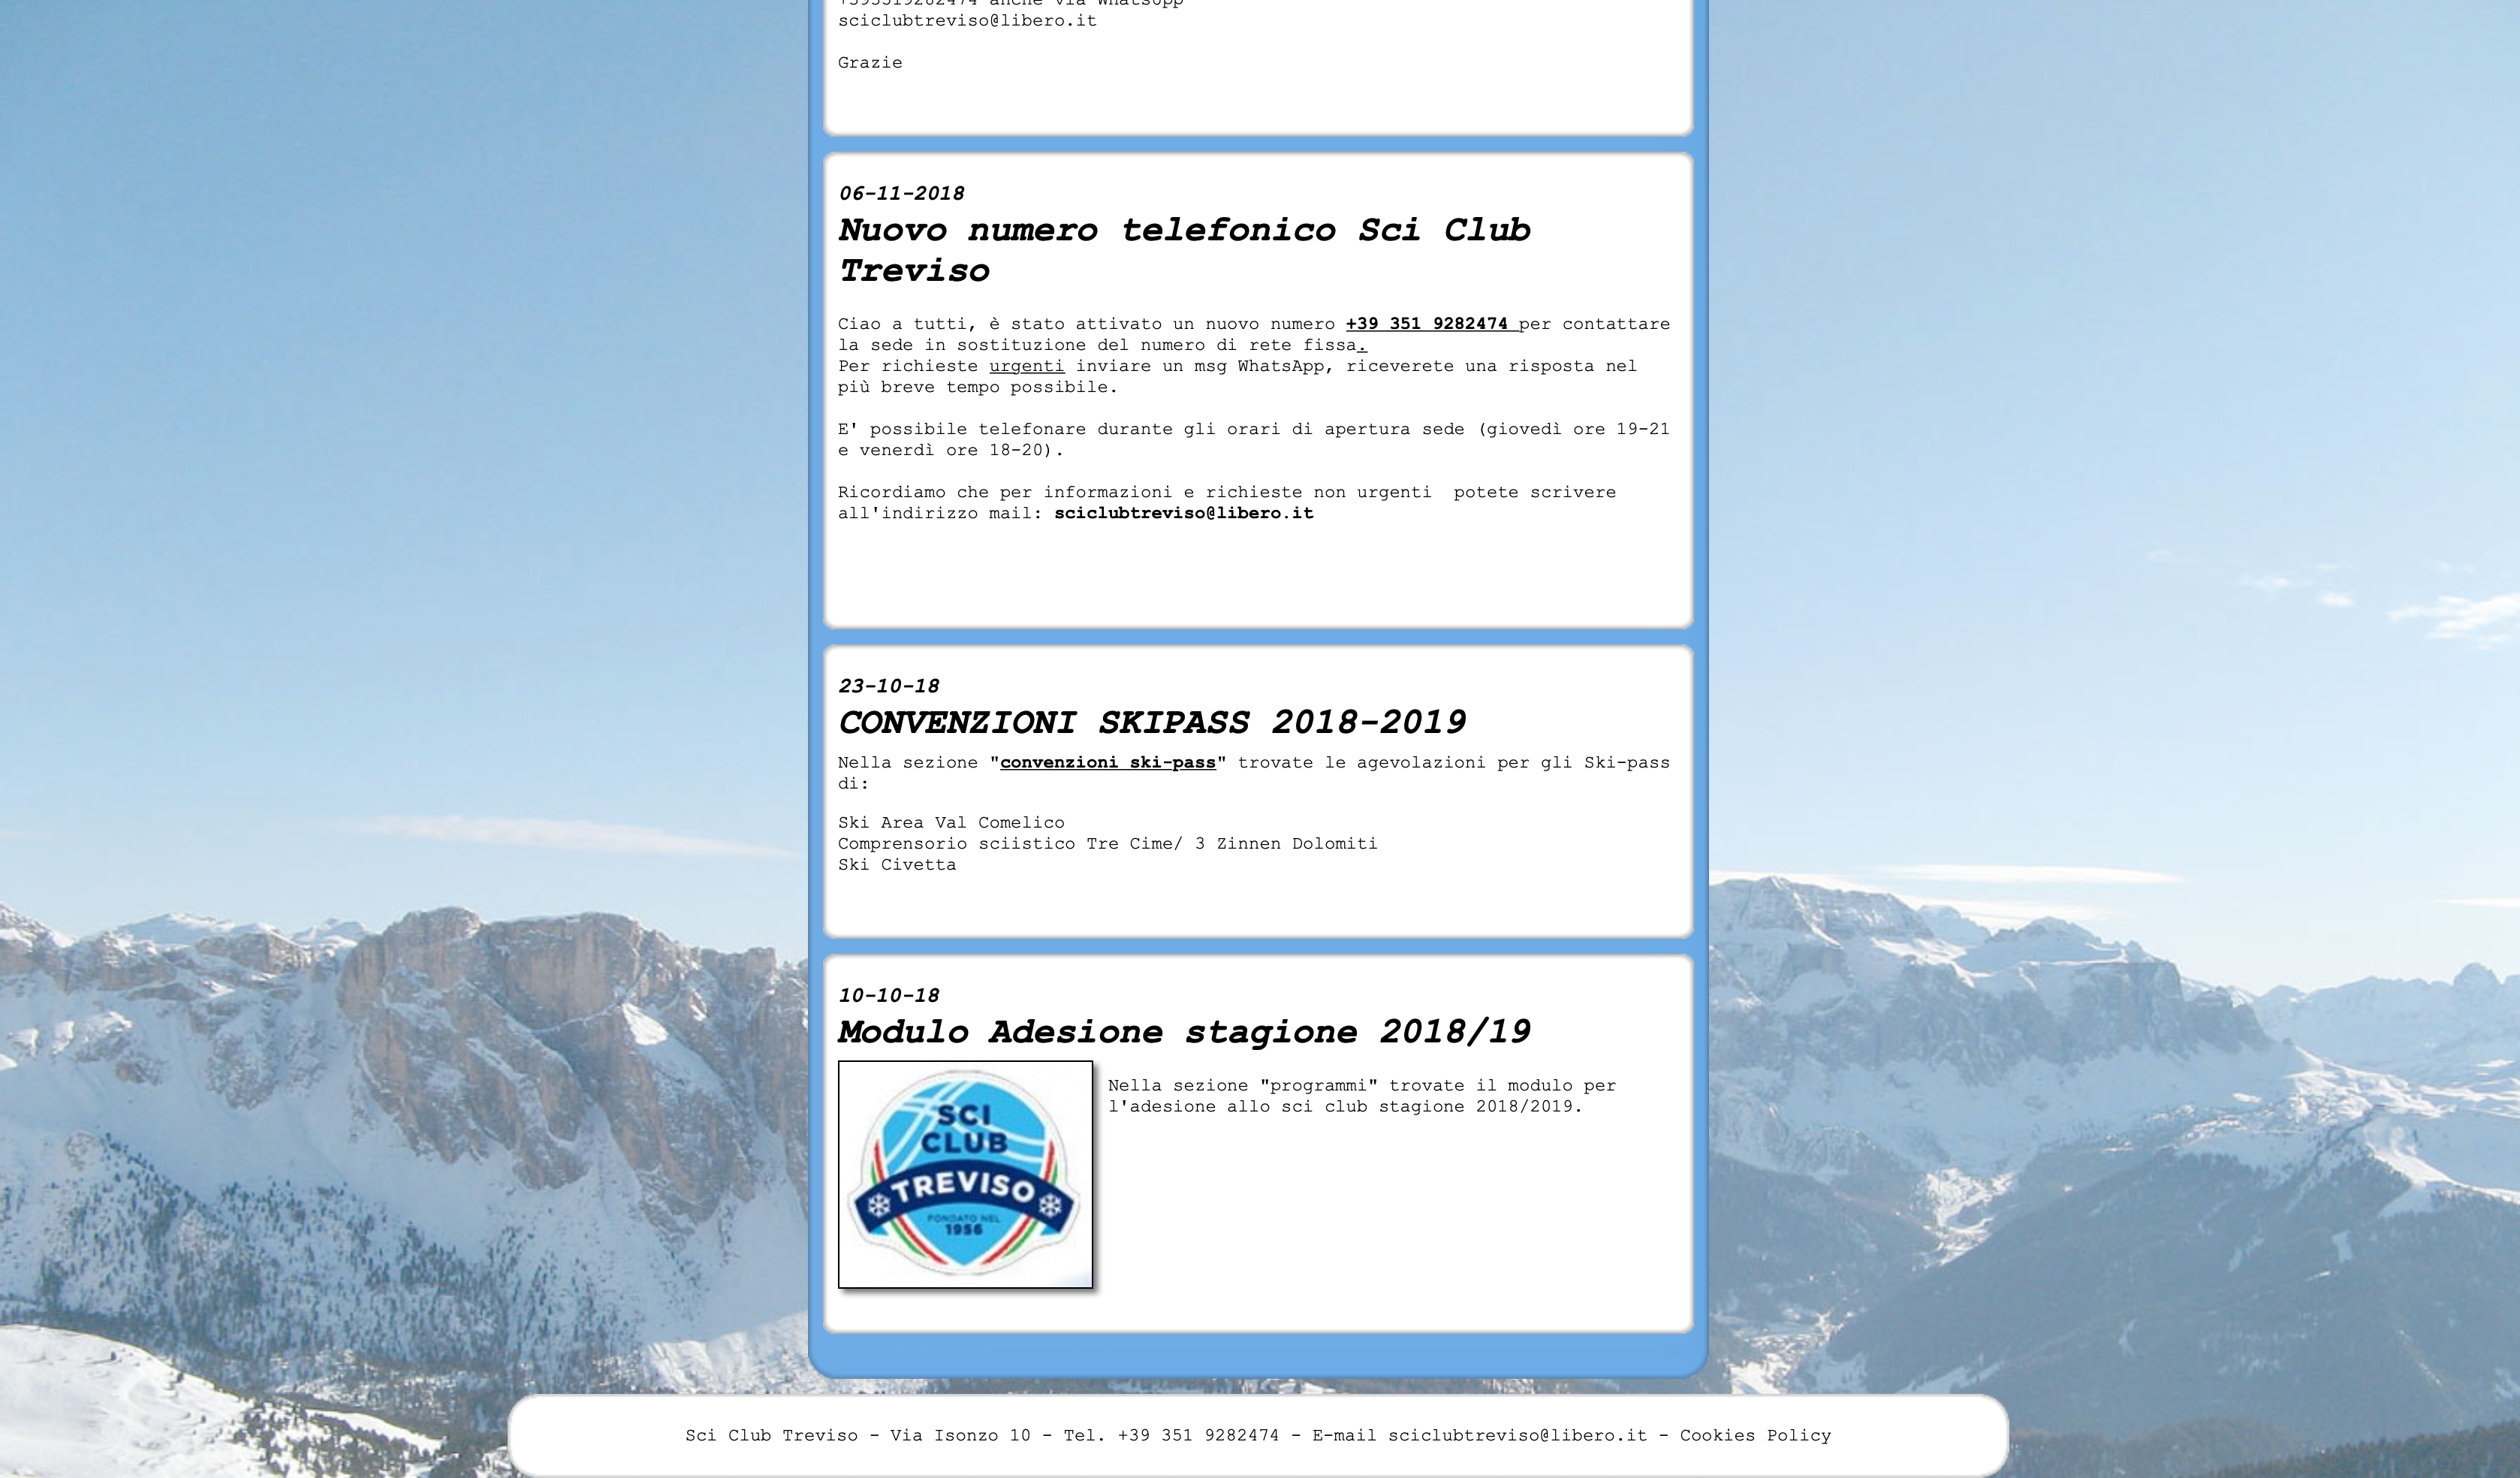
\includegraphics[width=.49\textwidth]{./immagini/homepage3}
    \caption [Homepage del sito 2]{Homepage del sito \siteName dopo scroll}
\end{figure}

    \subsection{Where}
        \begin{center}
            \textit{"A che tipo di sito sono arrivato?"}
        \end{center}
         Si capisce di essere nel sito dello Sci Club Treviso grazie ad un'immagine contente il logo e il nome dell'associazione, posta nella parte superiore della pagina, ma i due banner pubblicitari di due sponsor dell'associazione, fanno pensare diversamente. La prima volta che ho visitato questo sito pensavo di essere capitato nel sito sbagliato, dato che l'unica cosa che vedevo erano le pubblicità e non vi è alcuna altra informazione. 

    \subsection{Who}
        \begin{center}
            \textit{"Chi rappresenta il sito?"}
        \end{center}
        Per l'asse "Who" vale quanto detto nella sezione precedente: il logo e il nome dell'associazione soddisfano quest'asse ma la pubblicità invasiva 

    \subsection{Why}
    \begin{center}
        \textit{"Perché mai dovrei fermarmi su questo sito?"}
    \end{center}

    \subsection{What}
    \begin{center}
        \textit{"Cosa offre il sito?”}
    \end{center}

    \subsection{When}
    \begin{center}
        \textit{"Quali sono le ultime novità?”}
    \end{center}

    \subsection{How}
    \begin{center}
        \textit{"Come faccio ad arrivare alle sezioni principali?”}
    \end{center}

    
